\section{Ход работы}

Все результаты исследований приведены как вывод из консоли в конце отчёта.

Изначально была сгенерирована выборка $\epsilon_1, \ldots, \epsilon_n$, $n = 30$ из нормального распределения с $a = 0$ и $\sigma = 2$. Коэффициенты $\alpha$, $\beta_1$ и $\beta_2$ были получены случайно из промежутка $[0,1]$. Также был сгенерированы случайные числовые наборы $x_11, \ldots, x_1n$, $x_12, \ldots, x_n2$ со случаными параметрами математического ожидания и стандартного отклонения. После чего была сформирована выборка наблюдений $y_1, \ldots, y_n$ следующим образом:

\begin{equation}
	y_i = \alpha + \beta_1 \cdot x_{i1} + \beta_2 \cdot x_{i2} + \epsilon_i, i = \overline{1, n}
\end{equation}
Таким образом, исходные данные для последущего анализа являются значения показателя $y$ и объясняющих переменных $x_1$ и $x_2$.

Были построены парные линейные регрессии -- зависимости результативного признака $y$ от факторов, взятых по отдельности. Для каждой регрессии были построены поле корреляции с линией парной линейной регрессии и диаграммы остатков (остатки на фактор и остатки на номера наблюдений), а также вычислены коэффициенты уравнения линейной регрессии, коэффициент детерминации, коэффициент корреляции, величина средней ошибки аппроксимации. 

\begin{figure}[H]
	\begin{minipage}[H]{0.32\linewidth}
		\begin{center}
			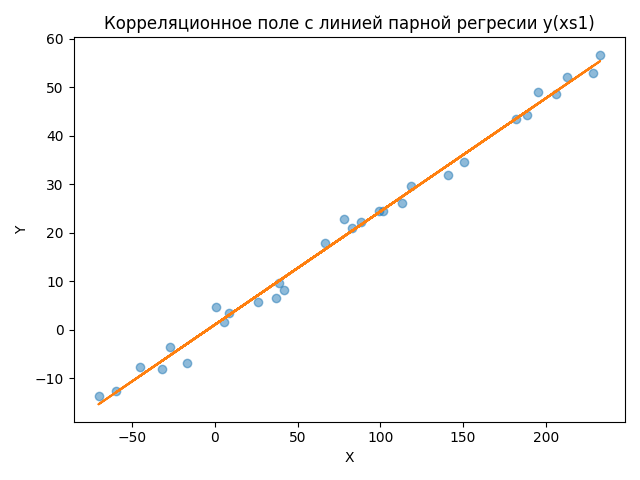
\includegraphics[width=\linewidth]{figures/scatter_xs1}
		\end{center}
	\end{minipage}
	\hfill
	\begin{minipage}[H]{0.32\linewidth}
		\begin{center}
			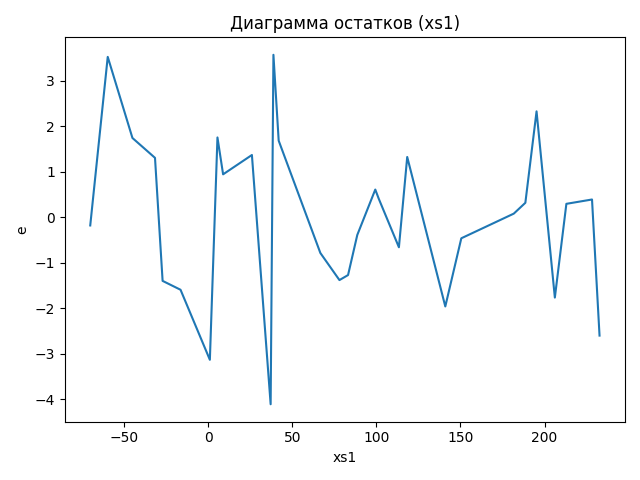
\includegraphics[width=\linewidth]{figures/res_plot_xs1}
		\end{center}
	\end{minipage}
	\hfill
	\begin{minipage}[H]{0.32\linewidth}
		\begin{center}
			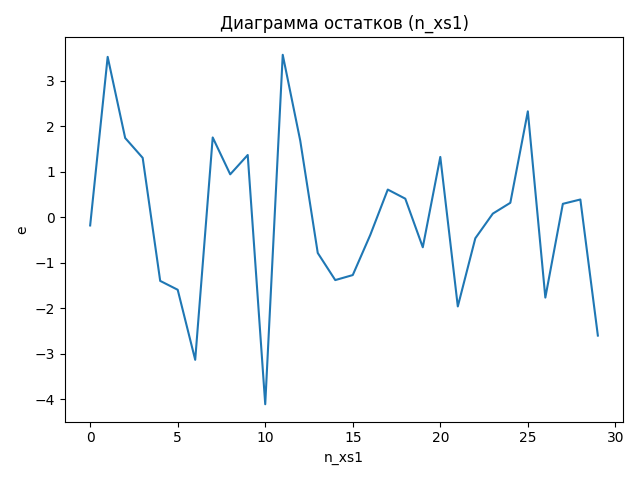
\includegraphics[width=\linewidth]{figures/res_plot_n_xs1}
		\end{center}
	\end{minipage}
\end{figure}

\begin{figure}[H]
	\begin{minipage}[H]{0.32\linewidth}
		\begin{center}
			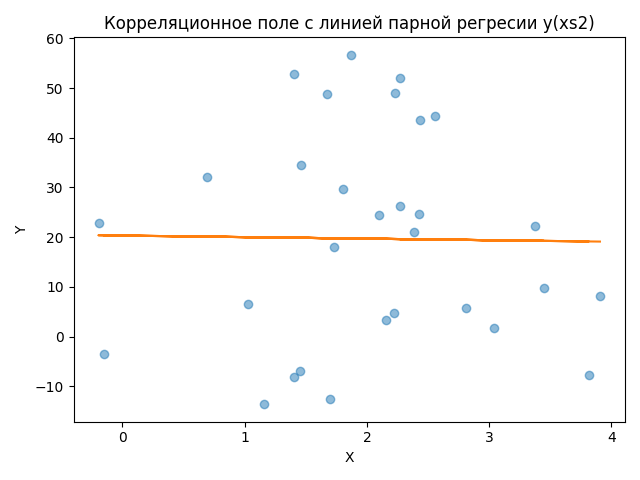
\includegraphics[width=\linewidth]{figures/scatter_xs2}
		\end{center}
	\end{minipage}
	\hfill
	\begin{minipage}[H]{0.32\linewidth}
		\begin{center}
			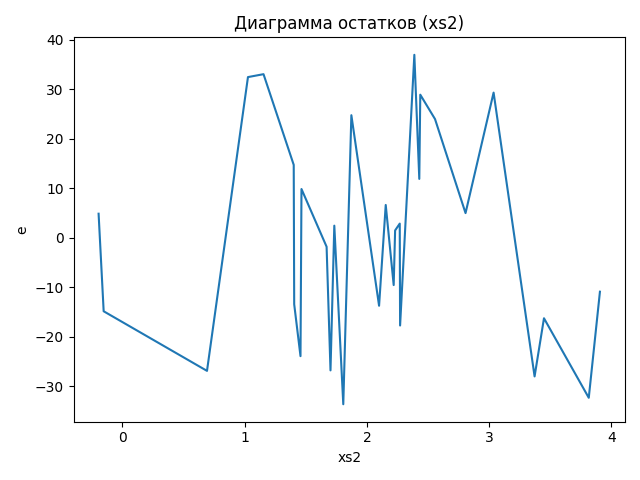
\includegraphics[width=\linewidth]{figures/res_plot_xs2}
		\end{center}
	\end{minipage}
	\hfill
	\begin{minipage}[H]{0.32\linewidth}
		\begin{center}
			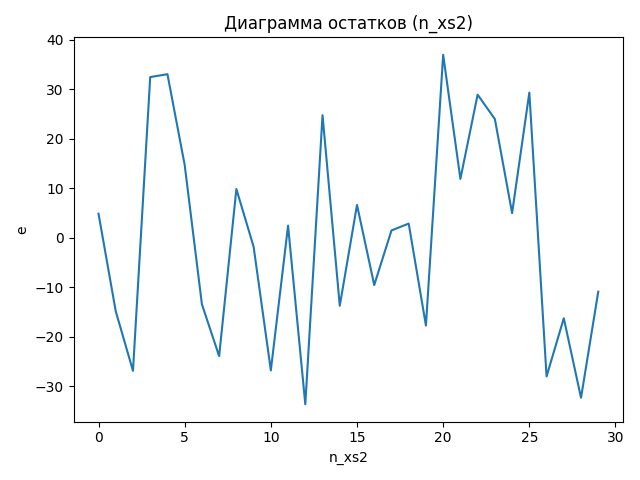
\includegraphics[width=\linewidth]{figures/res_plot_n_xs2}
		\end{center}
	\end{minipage}
\end{figure}


В соответствии с заданием были вычислены следующие параметры множественной регрессии:

\begin{itemize}

	\item Коэффициенты линейной регрессии
	\item Коэффициент корреляции
	\item Расчётные значения $\hat{y}_i = a + b \cdot x_i$, $i = \overline{1,n}$
	\item Отклонения $e_i = y_i - \hat{y}_i$, $i = \overline{1, n}$ истинных значений признака от расчётных
	\item Величина средней ошибки аппроксимации
	\item Оценка для дисперсии остатков
	\item Множественный коэффициент детерминации
	\item Фактическое значение $F$ критерия
	\item Частные коэффициенты корреляции в случае двух переменных
	\item Значения $t$-статистики для оценок $a$, $b_1$ и $b_2$. Также были сделаны выводы о статистической значимости данных коэффициентов.
	\item Точечный прогноз для индивидуального значения
	\item Интервальный прогноз

\end{itemize}

Также была построена диаграмма остатков на номера наблюдений для множественной регрессии:

\begin{figure}[H]
	\begin{minipage}[H]{\linewidth}
		\begin{center}
			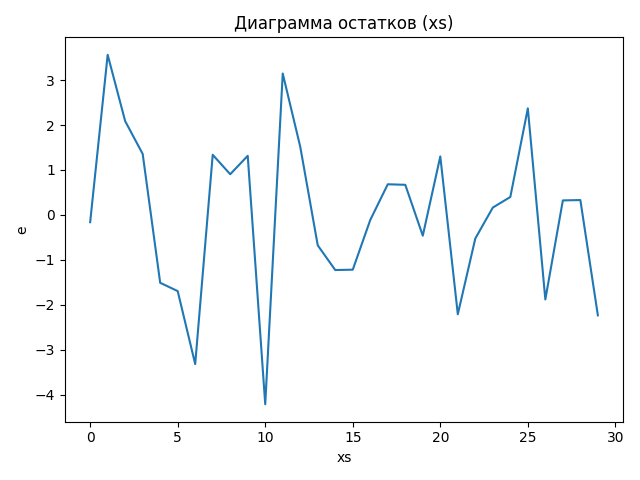
\includegraphics[width=\linewidth]{figures/res_plot_xs}
		\end{center}
	\end{minipage}
\end{figure}

Все вычисленные результаты представлены ниже.

\VerbatimInput{figures/file.txt}
